\chapter{Results and Discussion}

%The first set of experiments used the 'toy' artificial data set. 
%\bigskip

% The second set of
The experiments used the MNIST data set. In principle, any modern iteration of a \gls{cnn} can achieve very high accuracy on this data set \cite{mnist_sota_web}. \gls{nn}s ranging from simple CNNs to modern CapsNets, \gls{resnet}s and DenseNets (all \gls{dnn}s) should be able to achieve 98-99\% on this data set {\cite{mnist_sota_web}}. This is seen in the test and training accuracies in the baseline training schemes (figure \ref{fig:training_scheme_9_10}), where very high accuracies are achieved after only a few \gls{epoch}s. 
\bigskip

% https://tex.stackexchange.com/questions/140833/arranging-multiple-plots-in-a-grid-inside-a-figure-subfloat

% ZAMBINGO - include explanation of why CE test loss can't be calculated 

% ZAMBINGO - regenerate all plots to remove green/orange line....
% worst case scenario can shop them out - don't represent any actual data, just appended on

\begin{figure}[p]
    \centering
    \subfloat[Test accuracy]{
      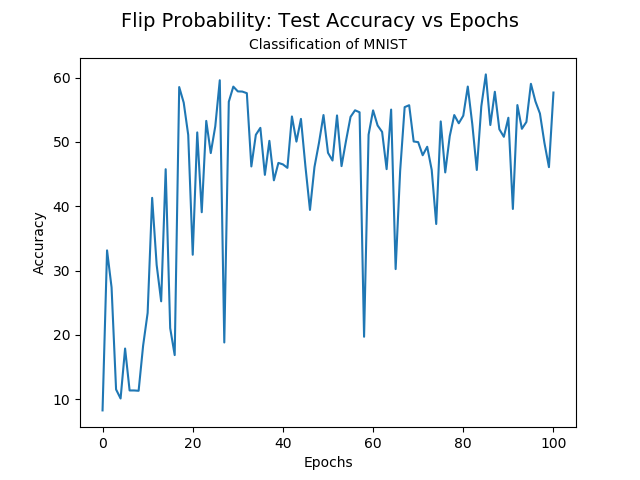
\includegraphics[width=65mm]{figs/run_1/test_accuracy_fp.png}
    }
    \subfloat[Flip probability loss - Test ]{
      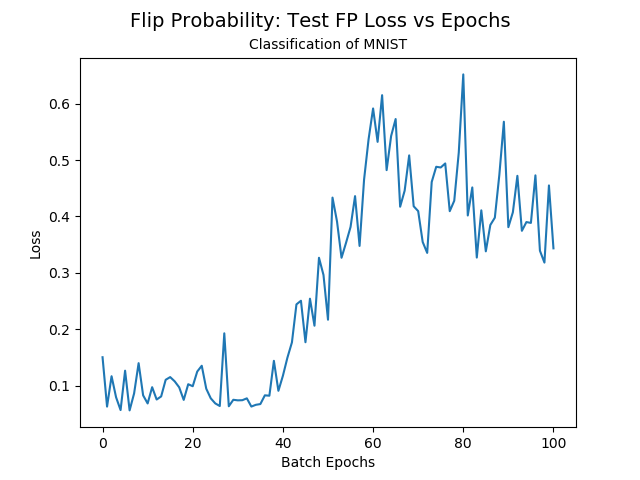
\includegraphics[width=65mm]{figs/run_1/test_losses_fp.png}
    }
    \hspace{0mm}
    \subfloat[Training accuracy]{
      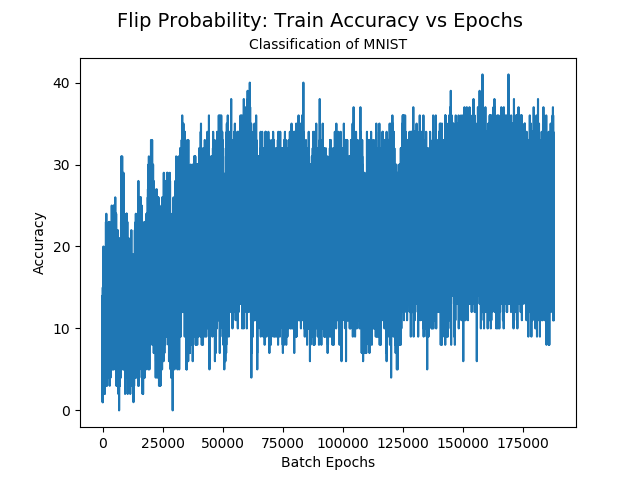
\includegraphics[width=65mm]{figs/run_1/train_accuracy.png}
    }
    \subfloat[Cross entropy loss]{
      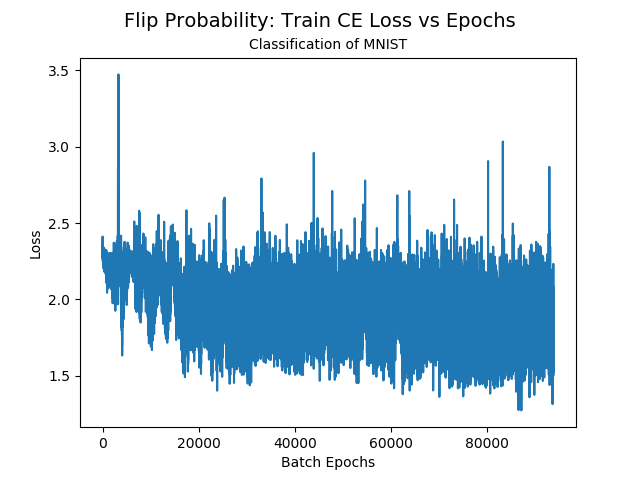
\includegraphics[width=65mm]{figs/run_1/train_losses_ce.png}
    }
    \hspace{0mm}
    \hbox to 67.5mm{}% !!
    \subfloat[Flip probability loss - training]{   % ???
      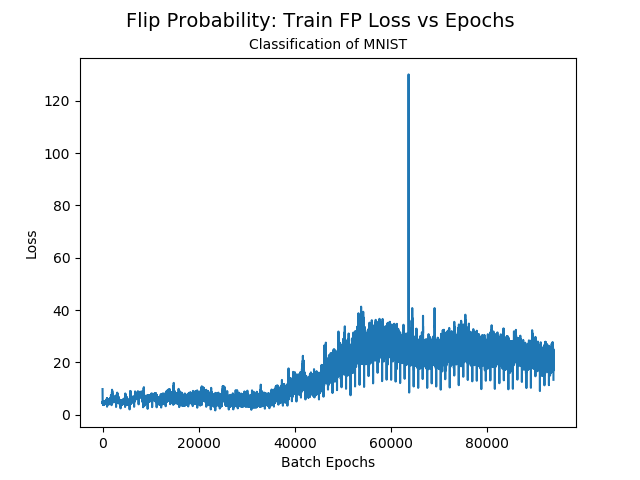
\includegraphics[width=65mm]{figs/run_1/train_losses_fp.png}
    }
    \caption[The results of the initial training scheme.]{The results of the initial training scheme, showing that the implementation has some promise, but has poor stability as training progresses.}
    \label{fig:training_scheme_1}
\end{figure}

The initial results in figure \ref{fig:training_scheme_1} show that using \gls{fp} as a \gls{lossfunction} is viable, if not very effective. We see that while the network sporadically achieves high test accuracies (often higher than the training accuracy's, although this effect would likely diminish once \gls{cv} is performed), the network settles in a low-accuracy configuration, where its performance on the test set is only equivalent to randomly guessing (10\% for the ten class case). It is possible the optimiser coasted past the local optimum on the loss surface, as we did not use a learning rate schedule to modulate the size of the steps towards the optimum as the algorithm is trained.
\bigskip

    
\begin{figure}[p]
    \centering
    \subfloat[Test accuracy]{
      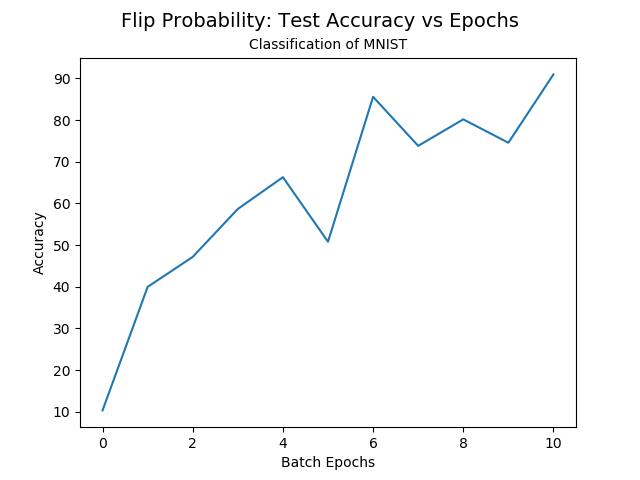
\includegraphics[width=65mm]{figs/run_2/test_accuracy_fp.png}
    }
    \subfloat[Flip probability loss - Test ]{
      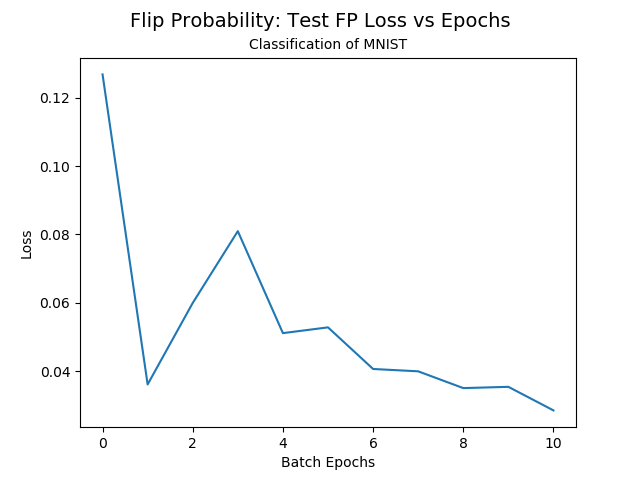
\includegraphics[width=65mm]{figs/run_2/test_losses_fp.png}
    }
    \hspace{0mm}
    \subfloat[Training accuracy]{
      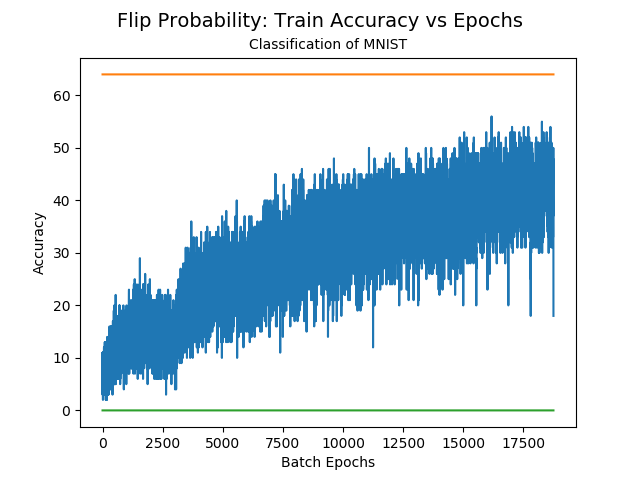
\includegraphics[width=65mm]{figs/run_2/train_accuracy.png}
    }
    \subfloat[Cross entropy loss]{
      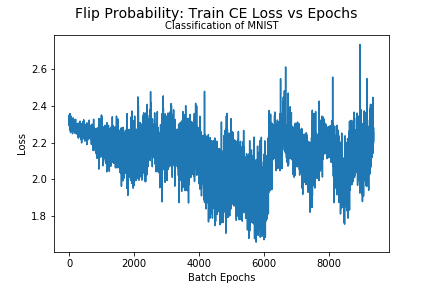
\includegraphics[width=65mm]{figs/run_2/train_losses_ce.png}
    }
    \hspace{0mm}
    \hbox to 67.5mm{}% !!
    \subfloat[Flip probability loss - training]{   % ???
      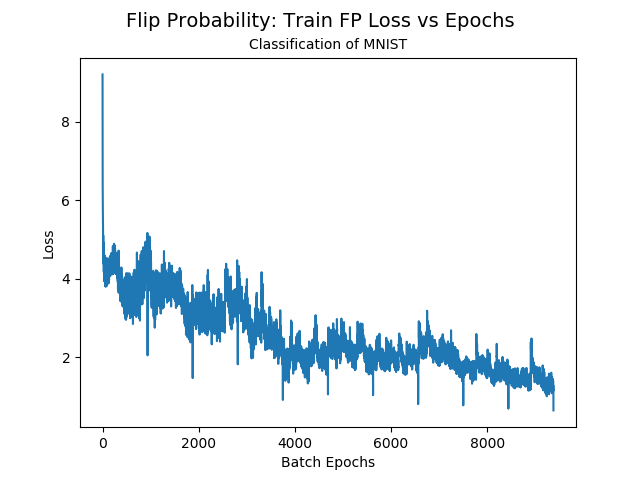
\includegraphics[width=65mm]{figs/run_2/train_losses_fp.png}
    }
    \caption[The results of the second training scheme.]{The results of the second training scheme, showing an improved performance over a short training span.}
    \label{fig:training_scheme_2}
\end{figure}

The results from training the algorithm for a shorter period of time (10 epochs) are more promising, although the test performance still pales in comparison to the baseline algorithm. We can see from the train accuracy and the loss graphs that there is a considerable amount of oscillation occurring when we switch from using the \gls{ce} loss to the \gls{fp} loss on a batc-wise basis. This likely comes from the problem of using two separate loss functions for the same modeling problem; as both loss functions would have a separate n-dimension surface they are being optimised on via \gls{sgd}, we are seeing a 'tug-of-war' as we alternate between them. It is possible that this also occurred with the initial training scheme (\ref{fig:training_scheme_1}) and there the algorithm ended up minimising the \gls{fp} loss preferentially to the \gls{ce} loss. However, as indicated by the loss plots, both are being minimised, although far more slowly than we might expect with using a single loss function. Extending the period of \gls{fp} training on the data worsens the results, as shown in \ref{fig:training_scheme_7}.
\bigskip

% Scheme 3 excluded from results as identical to run 4, sans training plot

%\begin{figure}[H]
%    \centering
%    \subfloat[Test Accuracy]{
%      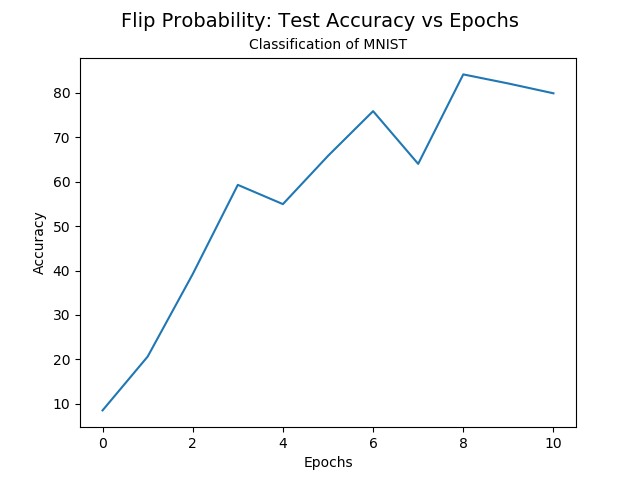
\includegraphics[width=65mm]{figs/run_3/test_accuracy_fp.png}
%    }
%    \subfloat[second]{
%      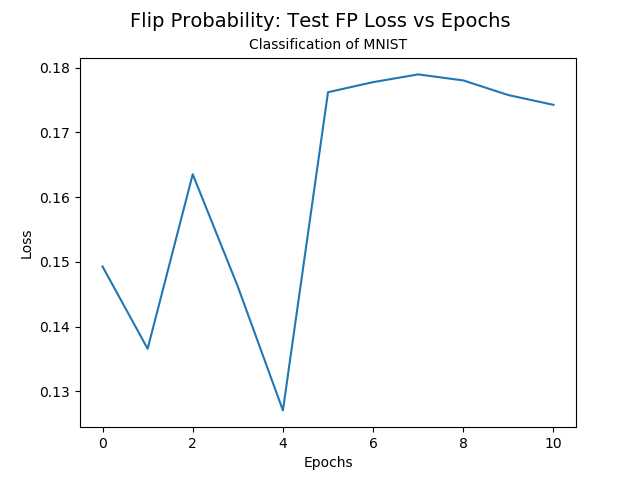
\includegraphics[width=65mm]{figs/run_3/test_losses_fp.png}
%    }
%    \hspace{0mm}
%    \subfloat[third]{
%      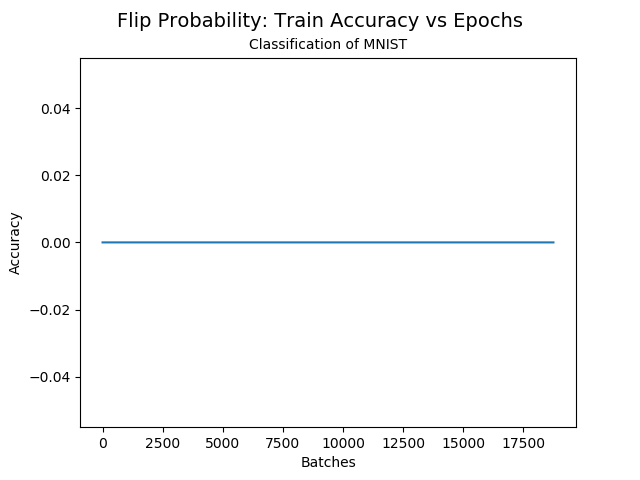
\includegraphics[width=65mm]{figs/run_3/train_accuracy.png}
%    }
%    \subfloat[Cross Entropy loss]{
%      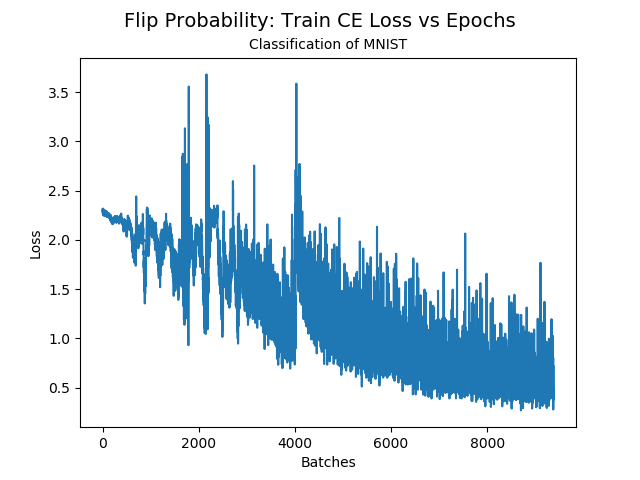
\includegraphics[width=65mm]{figs/run_3/train_losses_ce.png}
%    }
%    \hspace{0mm}
%    \hbox to 67.5mm{}% !!
%    \subfloat[Flip probability loss - Train]{   % ???
%      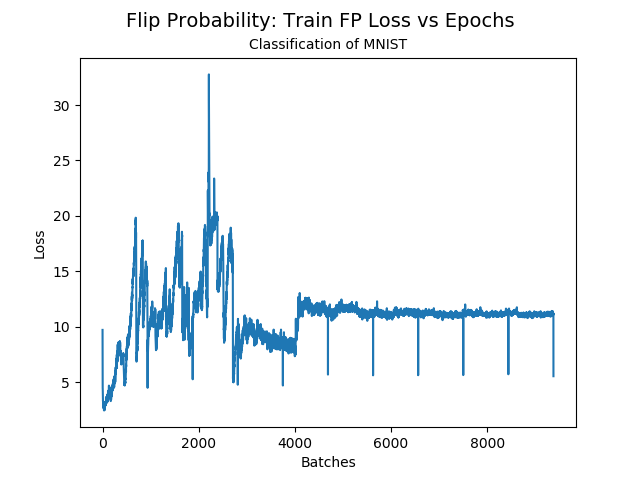
\includegraphics[width=65mm]{figs/run_3/train_losses_fp.png}
%    }
%    \caption{The results of the third training scheme}
%    \label{fig:training_scheme_3}
%\end{figure}

\begin{figure}[p]
    \centering
    \subfloat[Test accuracy]{
      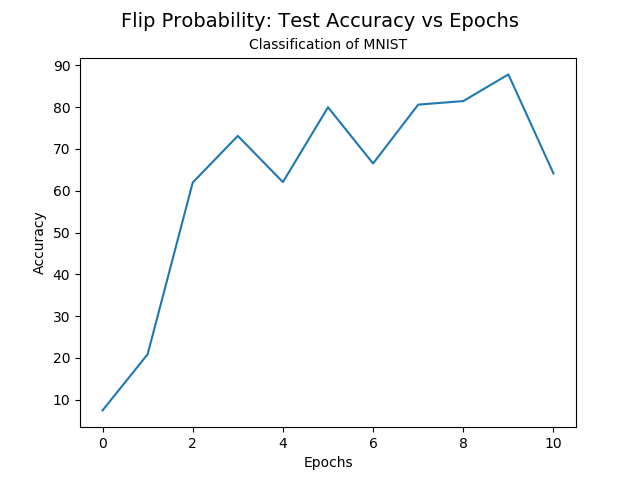
\includegraphics[width=65mm]{figs/run_4/test_accuracy_fp.png}
    }
    \subfloat[second]{
      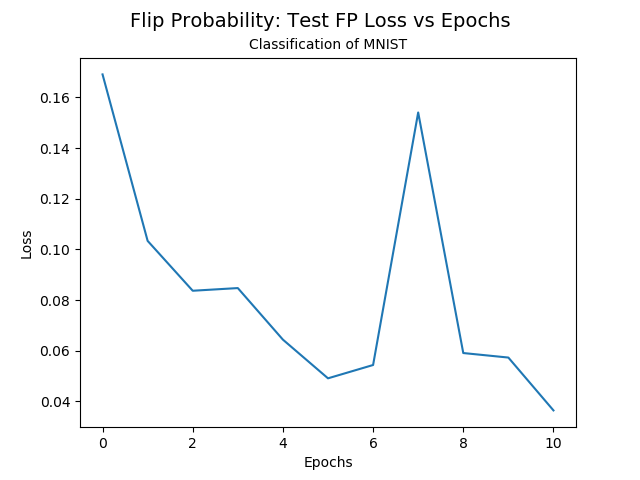
\includegraphics[width=65mm]{figs/run_4/test_losses_fp.png}
    }
    \hspace{0mm}
    \subfloat[Training accuracy]{
      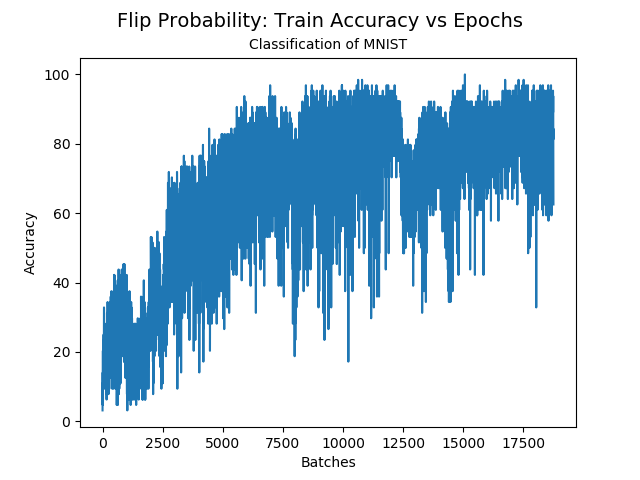
\includegraphics[width=65mm]{figs/run_4/train_accuracy.png}
    }
    \subfloat[Cross entropy loss]{
      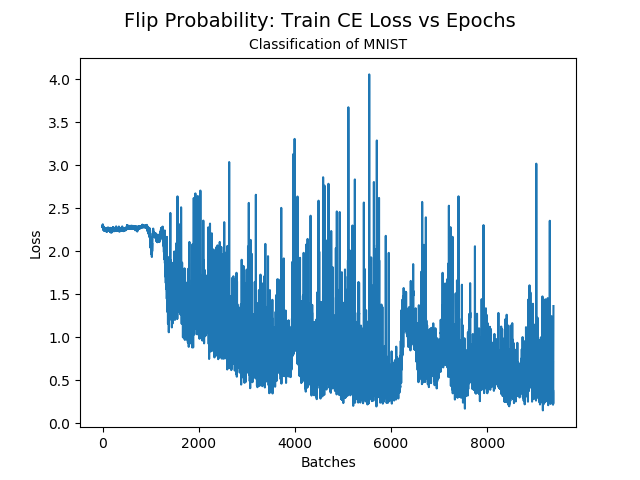
\includegraphics[width=65mm]{figs/run_4/train_losses_ce.png}
    }
    \hspace{0mm}
    \hbox to 67.5mm{}% !!
    \subfloat[Flip probability loss - train]{   % ???
      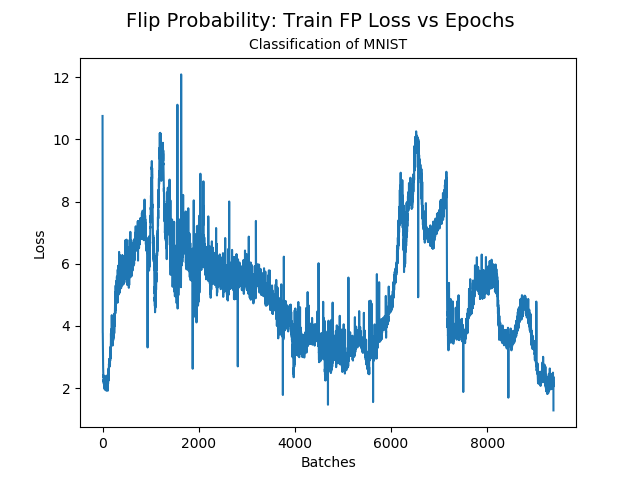
\includegraphics[width=65mm]{figs/run_4/train_losses_fp.png}
    }
    \caption[The results of the third training scheme.]{The results of the third training scheme, showing a high degree of instability in the loss functions when batch-wise alternation of the loss is used.}
    \label{fig:training_scheme_3}
\end{figure}



\begin{figure}[p]
    \centering
    \subfloat[Test accuracy]{
      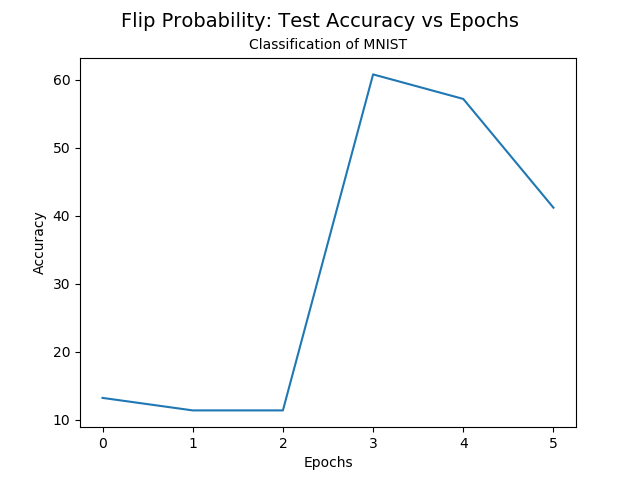
\includegraphics[width=65mm]{figs/run_5/test_accuracy_fp.png}
    }
    \subfloat[second]{
      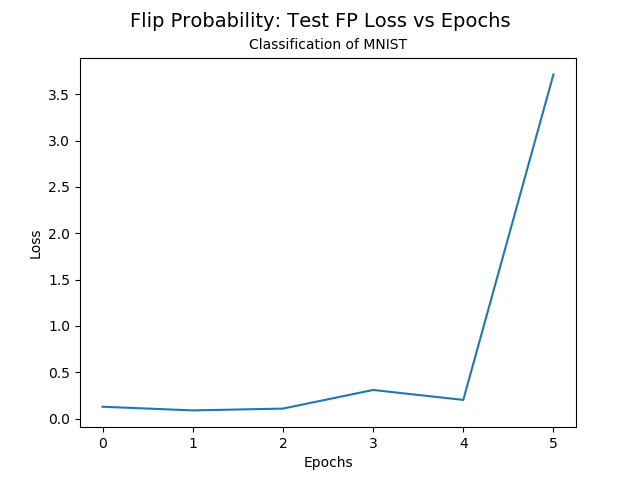
\includegraphics[width=65mm]{figs/run_5/test_losses_fp.png}
    }
    \hspace{0mm}
    \subfloat[Training accuracy]{
      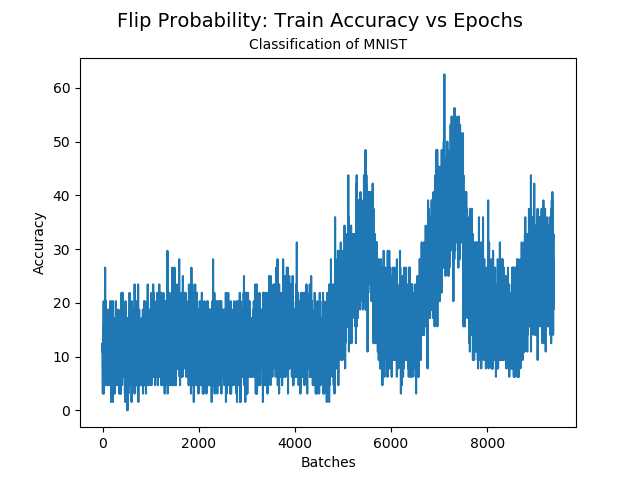
\includegraphics[width=65mm]{figs/run_5/train_accuracy.png}
    }
    \subfloat[Cross entropy loss]{
      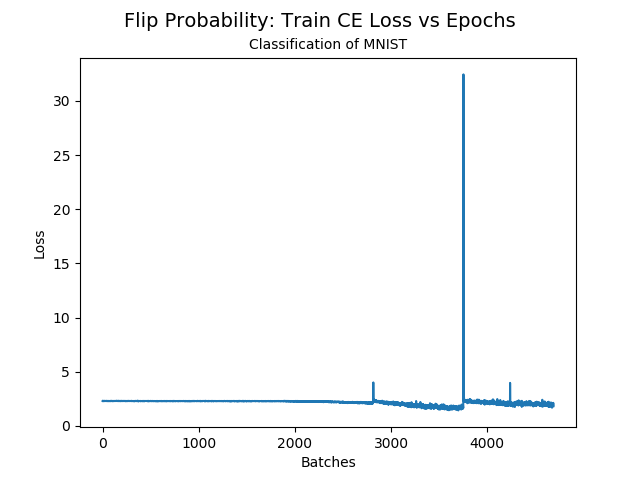
\includegraphics[width=65mm]{figs/run_5/train_losses_ce.png}
    }
    \hspace{0mm}
    \hbox to 67.5mm{}% !!
    \subfloat[Flip probability loss - training]{   % ???
      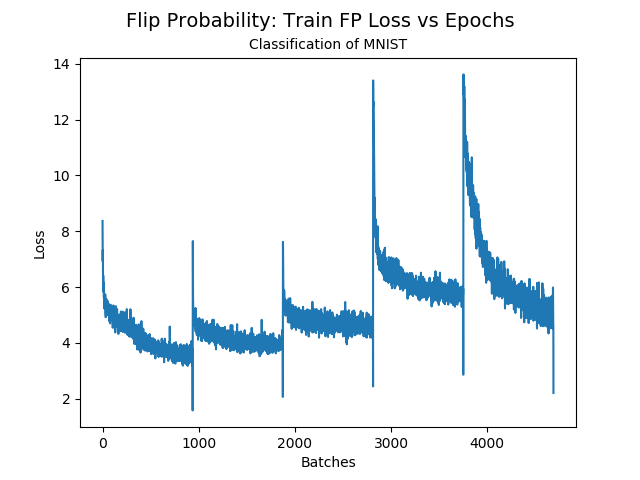
\includegraphics[width=65mm]{figs/run_5/train_losses_fp.png}
    }
    \caption[The results of the fourth training scheme]{The results of the fourth training scheme}
    \label{fig:training_scheme_4}
\end{figure}

% ZAMBINGO - reverse loss order and see if learning can occur (strictly speaking this shouldn't work).

\begin{figure}[p]
    \centering
    \subfloat[Test accuracy]{
      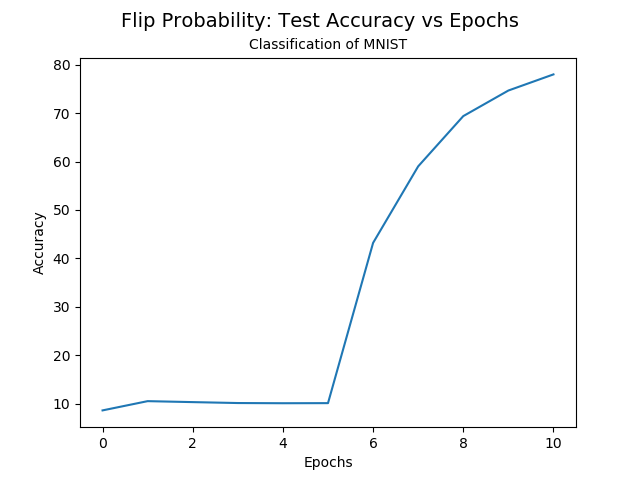
\includegraphics[width=65mm]{figs/run_6/test_accuracy_fp.png}
    }
    \subfloat[second]{
      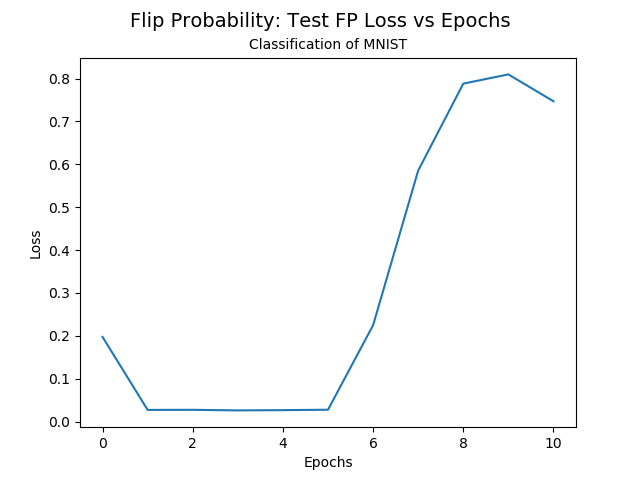
\includegraphics[width=65mm]{figs/run_6/test_losses_fp.png}
    }
    \hspace{0mm}
    \subfloat[Training accuracy]{
      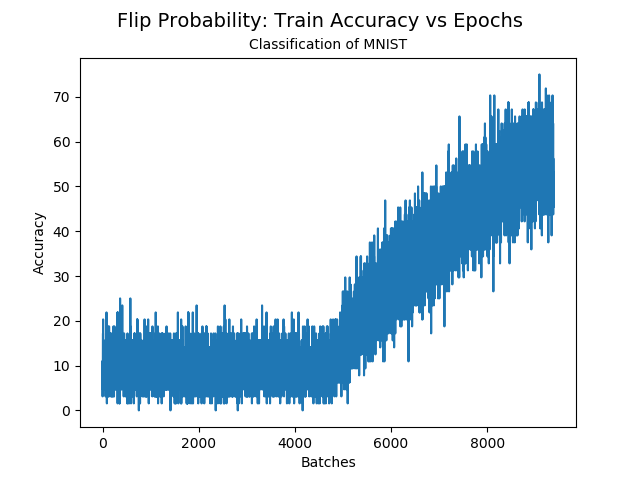
\includegraphics[width=65mm]{figs/run_6/train_accuracy.png}
    }
    \subfloat[Cross entropy loss]{
      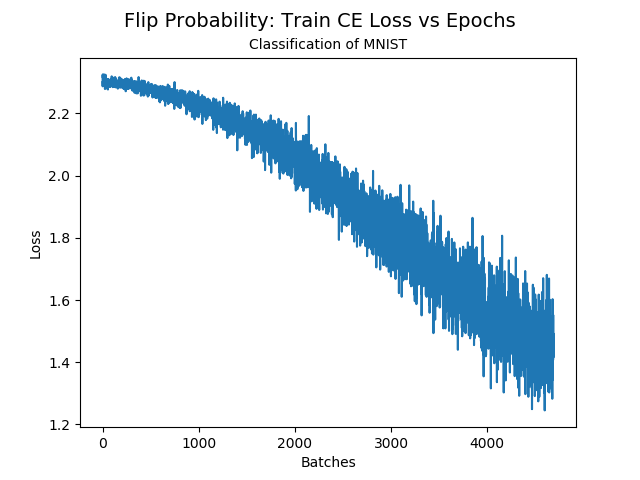
\includegraphics[width=65mm]{figs/run_6/train_losses_ce.png}
    }
    \hspace{0mm}
    \hbox to 67.5mm{}
    \subfloat[Flip probability loss - train]{   
      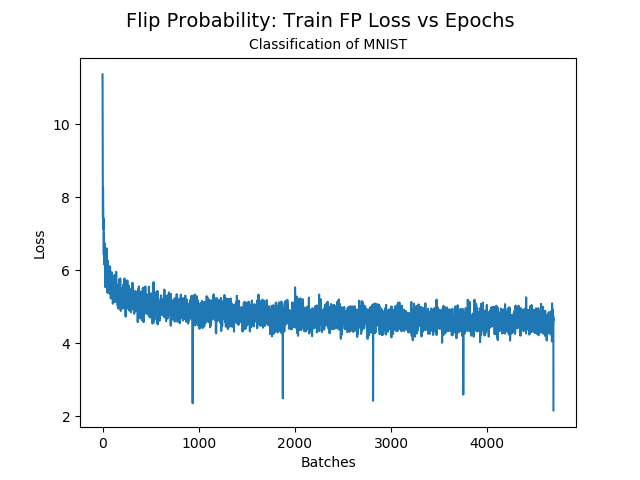
\includegraphics[width=65mm]{figs/run_6/train_losses_fp.png}
    }
    \caption[The results of the fifth training scheme]{The fifth training scheme shows that once the loss is switched to \gls{fp}, the \gls{ce} loss rapidly decreases and test and training training accuracy increase, although not to baseline levels. The \gls{fp} loss shows the first half of training batches, while the \gls{ce} loss shows the second half.}
    \label{fig:training_scheme_5}
\end{figure}

\begin{figure}[p]
    \centering
    \subfloat[Test accuracy]{
      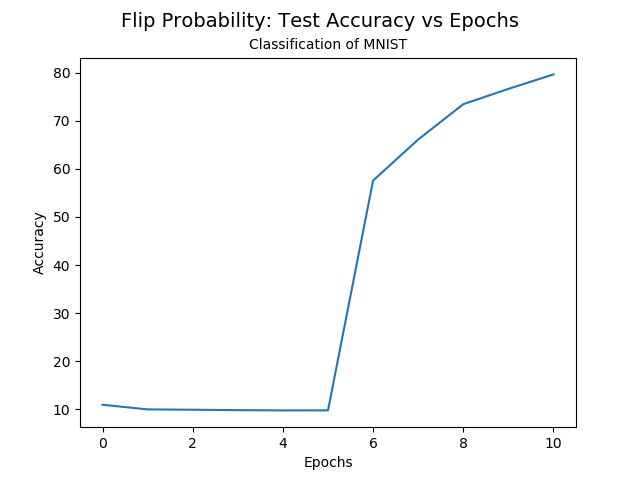
\includegraphics[width=65mm]{figs/run_7/test_accuracy_fp.png}
    }
    \subfloat[Flip probability loss - Test ]{
      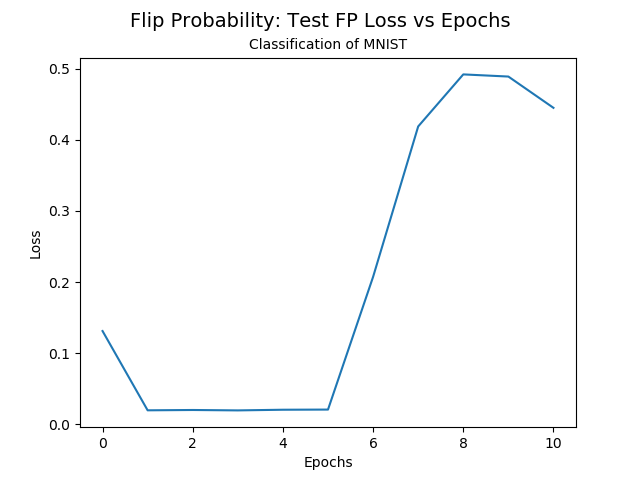
\includegraphics[width=65mm]{figs/run_7/test_losses_fp.png}
    }
    \hspace{0mm}
    \subfloat[Training accuracy]{
      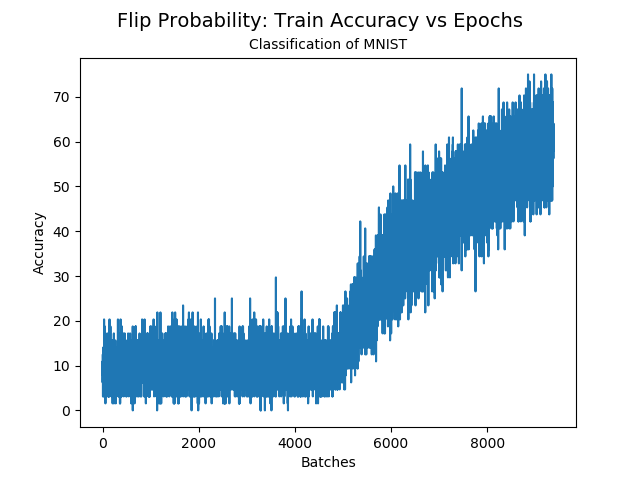
\includegraphics[width=65mm]{figs/run_7/train_accuracy.png}
    }
    \subfloat[Cross entropy loss]{
      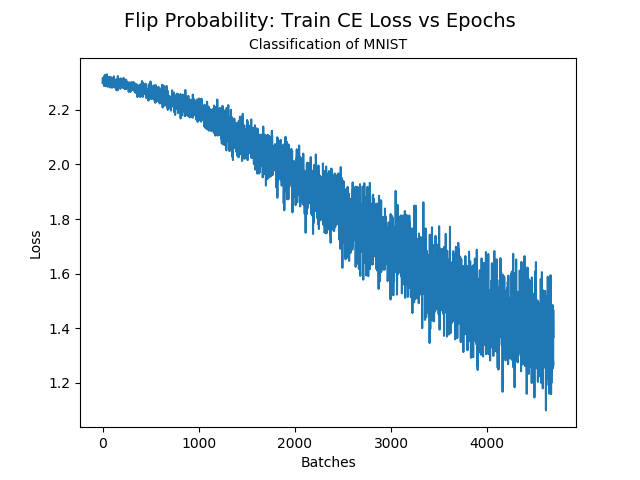
\includegraphics[width=65mm]{figs/run_7/train_losses_ce.png}
    }
    \hspace{0mm}
    \hbox to 67.5mm{}
    \subfloat[Flip probability loss - train]{  
      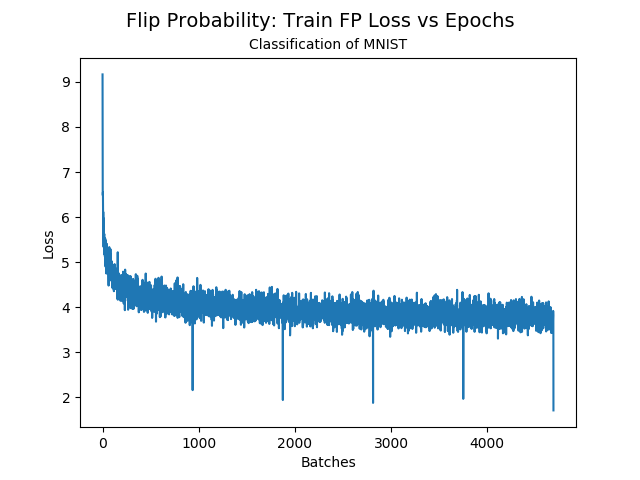
\includegraphics[width=65mm]{figs/run_7/train_losses_fp.png}
    }
    \caption[The results of the sixth training scheme]{The results of the sixth training scheme show using momentum has no significant effect on the results.}
    \label{fig:training_scheme_6}
\end{figure}

\begin{figure}[p]
    \centering
    \subfloat[Test accuracy]{
      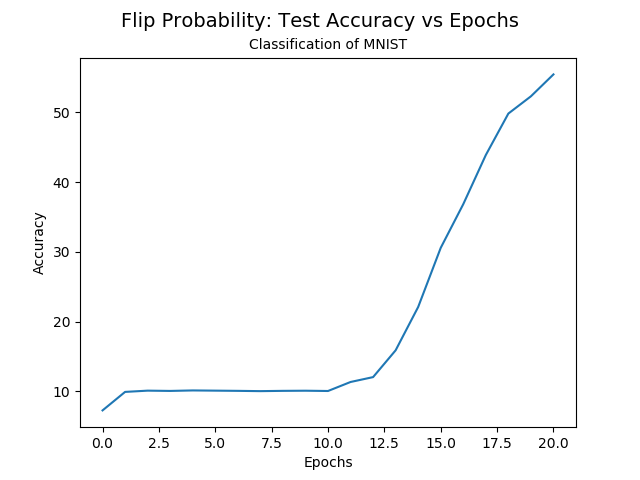
\includegraphics[width=65mm]{figs/run_8/test_accuracy_fp.png}
    }
    \subfloat[Flip probability loss - Test ]{
      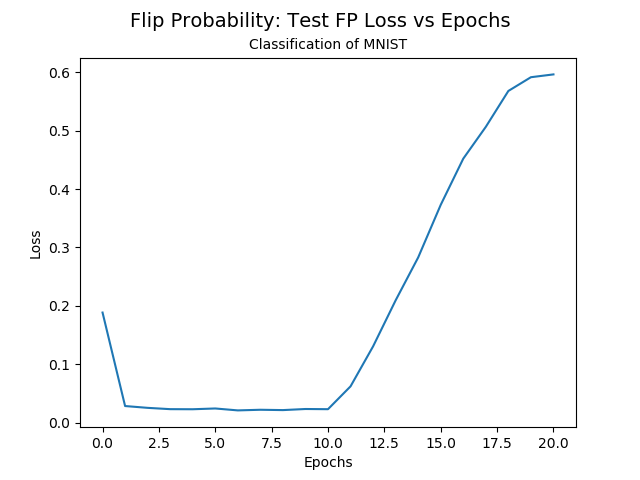
\includegraphics[width=65mm]{figs/run_8/test_losses_fp.png}
    }
    \hspace{0mm}
    \subfloat[Training accuracy]{
      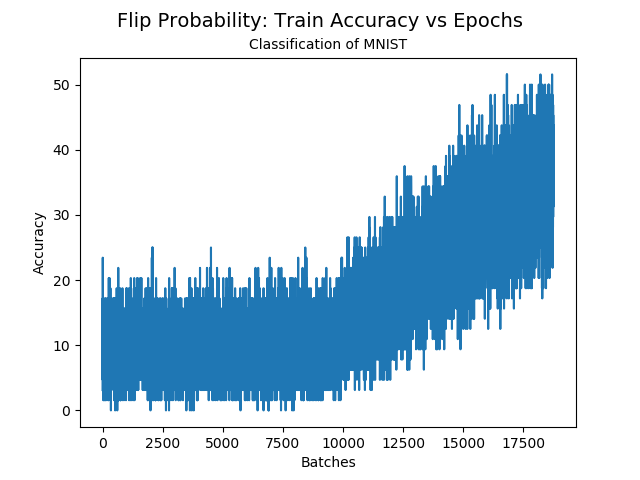
\includegraphics[width=65mm]{figs/run_8/train_accuracy.png}
    }
    \subfloat[Cross entropy loss]{
      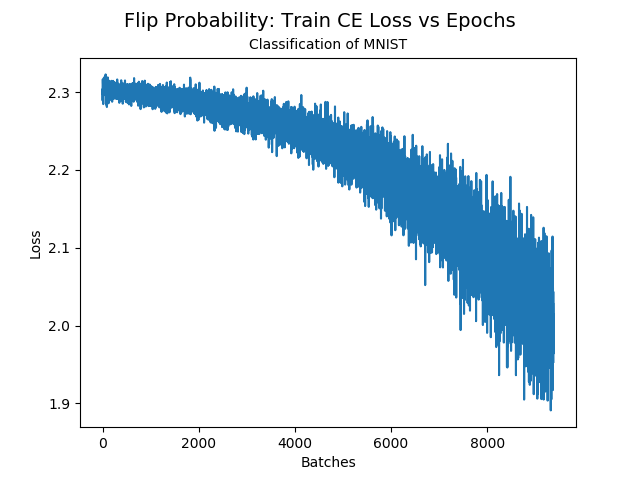
\includegraphics[width=65mm]{figs/run_8/train_losses_ce.png}
    }
    \hspace{0mm}
    \hbox to 67.5mm{}
    \subfloat[Flip probability loss - training]{
      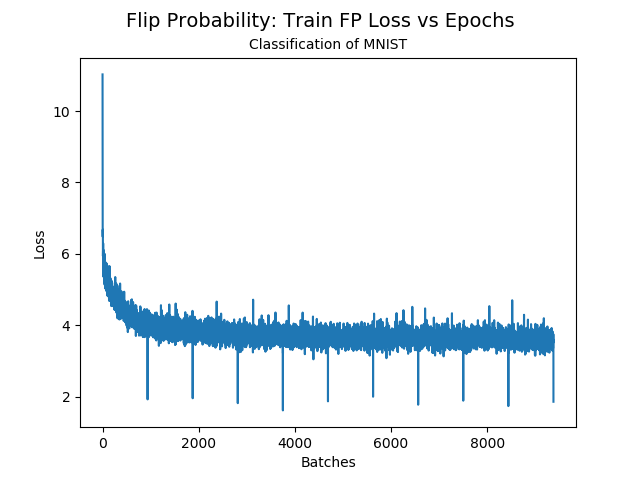
\includegraphics[width=65mm]{figs/run_8/train_losses_fp.png}
    }
    \caption[The results of the seventh training scheme]{The seventh training scheme shows that extending the period of representation training to 10 epochs worsens the results when the regular learning process using \gls{ce} is resumed.}
    \label{fig:training_scheme_7}
\end{figure}

\begin{figure}[p]
    \centering
    \subfloat[Test accuracy]{
      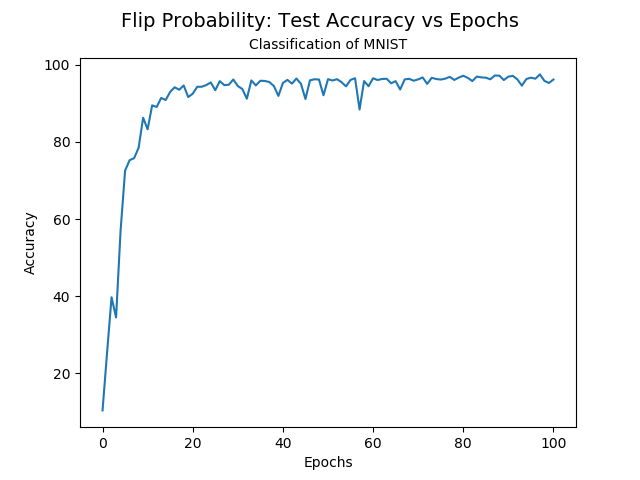
\includegraphics[width=65mm]{figs/run_9/test_accuracy_fp.png}
    }
    \subfloat[Flip probability loss - testing]{
      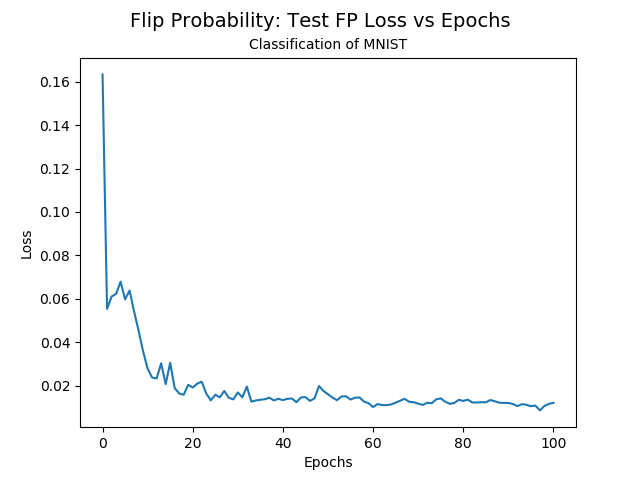
\includegraphics[width=65mm]{figs/run_9/test_losses_fp.png}
    }
    \hspace{0mm}
    \subfloat[Training accuracy]{
      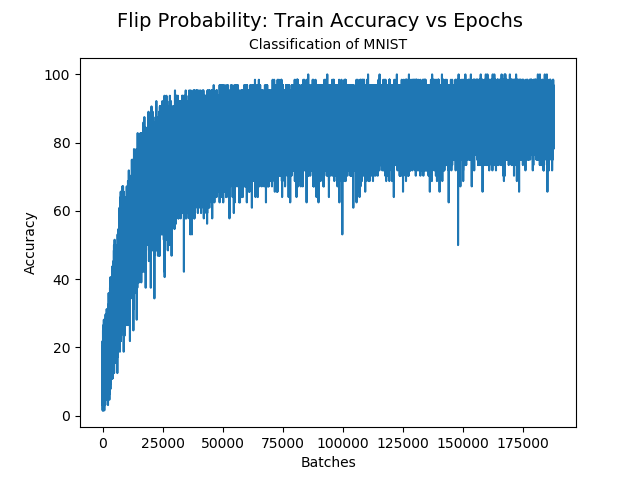
\includegraphics[width=65mm]{figs/run_9/train_accuracy.png}
    }
    \subfloat[Cross entropy loss]{
      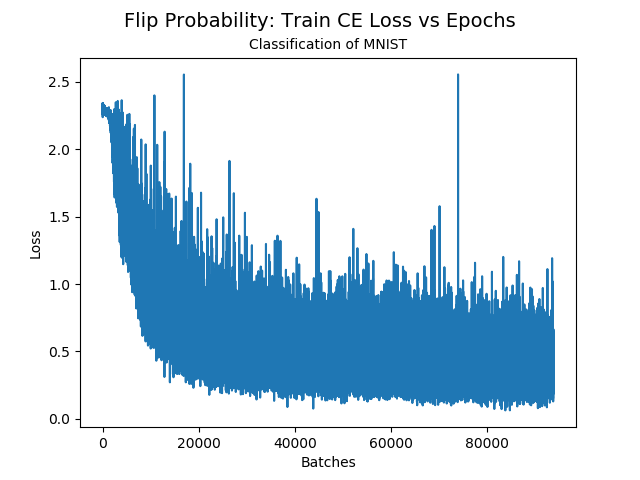
\includegraphics[width=65mm]{figs/run_9/train_losses_ce.png}
    }
    \hspace{0mm}
    \hbox to 67.5mm{}
    \subfloat[Flip probability loss - train]{   
      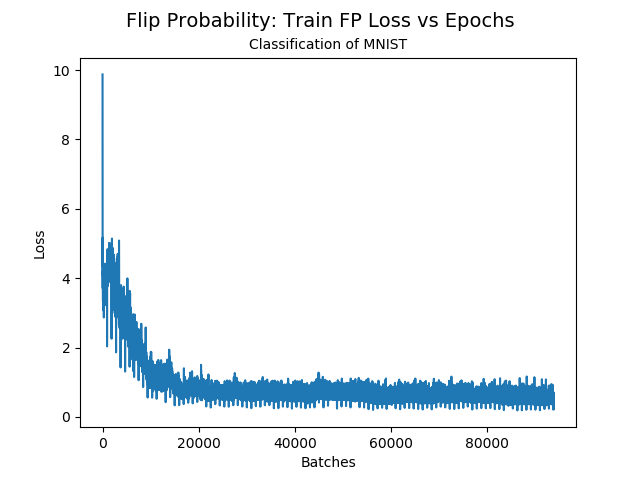
\includegraphics[width=65mm]{figs/run_9/train_losses_fp.png}
    }
    \caption[The results of the eighth training scheme]{Setting up the training procedure such that the network alernates between training mostly on \gls{ce} loss and only trains on \gls{fp} loss for short periods improves performance considerably, suggesting \gls{fp} has a detrimental effect.}
    \label{fig:training_scheme_8}
\end{figure}

\newpage

%\newgeometry{top=1cm}

\begin{figure}[p]
    \centering
    \subfloat[Test Accuracy - normalised]{
      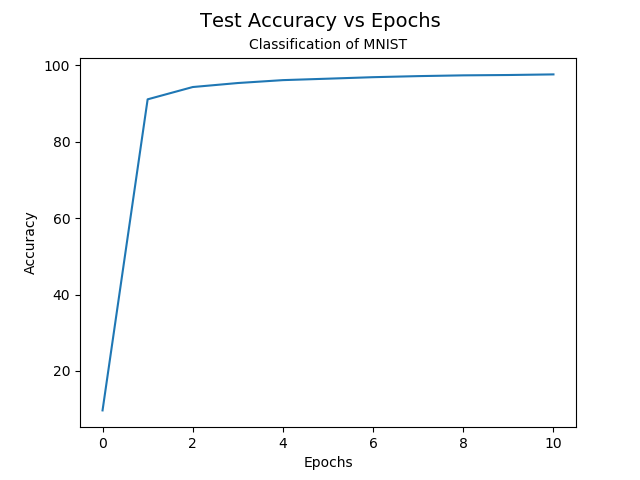
\includegraphics[width=50mm]{figs/run_10/test_accuracy_fp.png}
    }
    \subfloat[Cross Entropy loss - normalised]{
      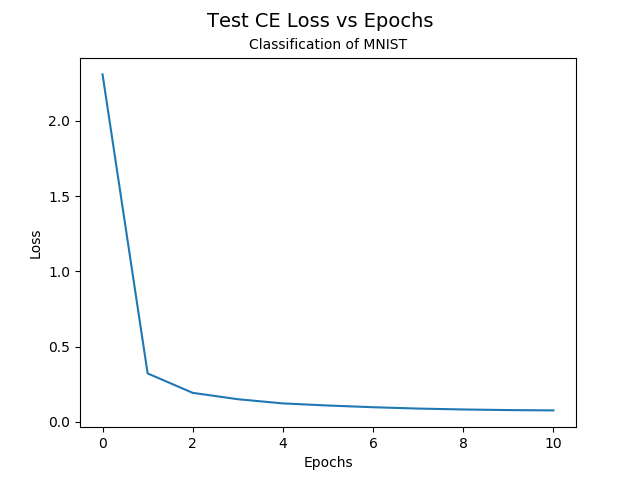
\includegraphics[width=50mm]{figs/run_10/test_losses_fp.png}
    }
    \hspace{0mm}
    \subfloat[Train Accuracy - normalised]{
      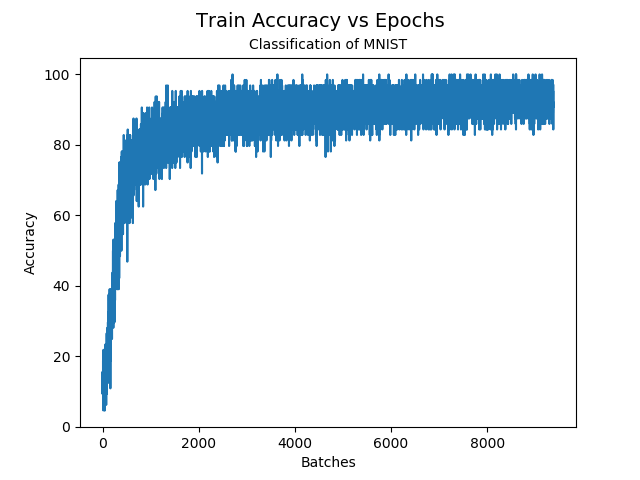
\includegraphics[width=50mm]{figs/run_10/train_accuracy.png}
    }
    \subfloat[Train Cross Entropy loss - normalised]{
      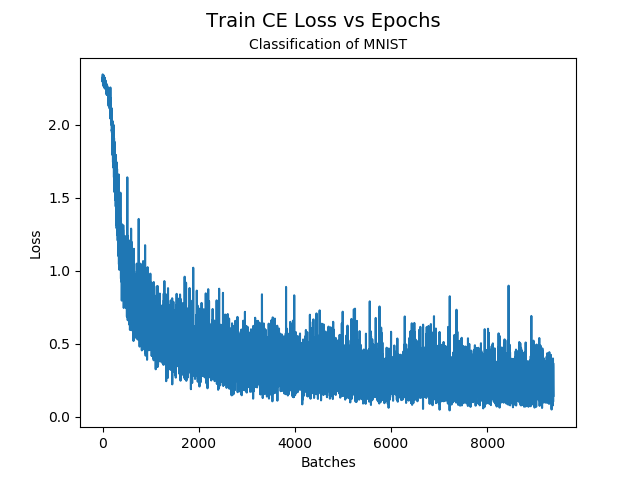
\includegraphics[width=50mm]{figs/run_10/train_losses_ce.png}
    }
    \hspace{0mm}
    \subfloat[Test Accuracy - no normalisation]{
      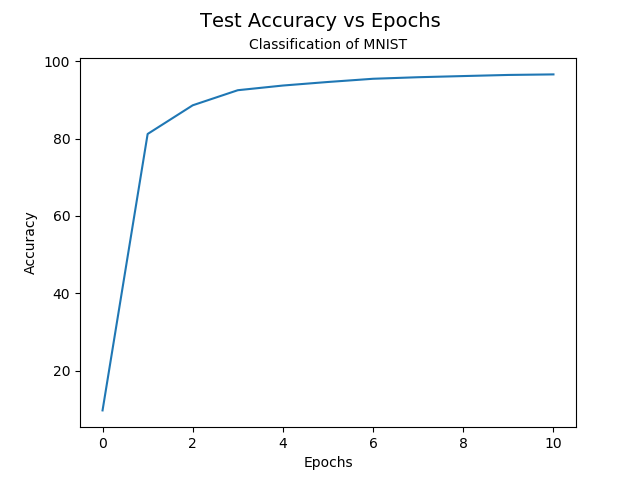
\includegraphics[width=50mm]{figs/run_11/test_accuracy_fp.png}
    }
    \subfloat[Cross Entropy loss - no normalisation]{
      \includegraphics[width=50mm]{figs/run_11/test_losses_fp.png}
    }
    \hspace{0mm}
    \subfloat[Train Accuracy - no normalisation]{
      \includegraphics[width=50mm]{figs/run_11/train_accuracy.png}
    }
    \subfloat[Train Cross Entropy loss - no normalisation]{
      \includegraphics[width=50mm]{figs/run_11/train_losses_ce.png}
    }
    \hspace{0mm}
    \caption[The results of the ninth and tenth training scheme, the baseline scheme, with and without normalisation]{The baseline scheme, both with normalised and unnormalised input data, showing very high test accuracies after only a few epochs.}
    \label{fig:training_scheme_9_10}
\end{figure}

%\restoregeometry

%\begin{figure}
%\centering
%
%
%\caption{The results of the eleventh training scheme, the baseline with no normalisation}
%\label{fig:training_scheme_11}
%\end{figure}

\begin{figure}[p]
    \centering
    \subfloat[Test accuracy]{
      \includegraphics[width=65mm]{figs/run_12/test_accuracy_fp.png}
    }
    \subfloat[Flip probability loss - testing]{
      \includegraphics[width=65mm]{figs/run_12/test_losses_fp.png}
    }
    \hspace{0mm}
    \subfloat[Training accuracy]{
      \includegraphics[width=65mm]{figs/run_12/train_accuracy.png}
    }
    \subfloat[Cross entropy loss]{
      \includegraphics[width=65mm]{figs/run_12/train_losses_ce.png}
    }
    \hspace{0mm}
    \hbox to 67.5mm{}% !!
    \subfloat[Flip probability loss - training]{   % ???
      \includegraphics[width=65mm]{figs/run_12/train_losses_fp.png}
    }
    \caption{The results of the eleventh training scheme}
    \label{fig:training_scheme_11}
\end{figure}

\begin{figure}[p]
    \centering
    \subfloat[Test accuracy]{
      \includegraphics[width=65mm]{figs/run_13/test_accuracy_fp.png}
    }
    \subfloat[Flip probability loss - testing]{
      \includegraphics[width=65mm]{figs/run_13/test_losses_fp.png}
    }
    \hspace{0mm}
    \subfloat[Training accuracy]{
      \includegraphics[width=65mm]{figs/run_13/train_accuracy.png}
    }
    \subfloat[Cross entropy loss]{
      \includegraphics[width=65mm]{figs/run_13/train_losses_ce.png}
    }
    \hspace{0mm}
    \hbox to 67.5mm{}% !!
    \subfloat[Flip probability loss - training]{   % ???
      \includegraphics[width=65mm]{figs/run_13/train_losses_fp.png}
    }
    \caption[The results of the twelfth training scheme]{Running the network for many epochs with \gls{fp} loss, without momentum or drop-out shows results that are at least comparable to the baseline scheme, given sufficient training time.}
    \label{fig:training_scheme_12}
\end{figure}

We can see that the baseline schemes (figure \ref{fig:training_scheme_9_10}), clearly achieve a very high accuracy rapidly with minimal oscillation. Removing image normalisation slightly decreases training and testing accuracy during the early stages of training, but otherwise has little effect on the final accuracy.
\bigskip

%The third, more refined set of experiments was on the \gls{cifar}-10 data set
%\bigskip
%
%The final experiment was an attempt to implement \gls{fp} in a \gls{dl} context, to see if any %improvements could be made. We used the Tiny ImageNet data set
%\bigskip